% En la figura \ref{fig:con_paralelizacion_datos} se presenta la misma
% aplicación (esta vez se la denomina \textit{app}). En este ejemplo
% los datos representados por $D$ anteriomente, se
% dividien en $D_{n}$ secciones más pequeñas que son distribuidas a distintos
% núcleos de procesamiento \footnote{en el ejemplo se utilizan 4, aunque pueden ser más
% núcleos dentro de un procesador}. Una copia idéntica de la aplicación (Figura
% \ref{fig:sin_paralelizacion_datos}) se encuentra corriendo en cada uno de los
% cuatro núcleos del ordenador, cada una de estas copias idénticas se
% encuentra trabajando con datos distintos (ya que a cada una de las copias le
% toca una sección $D_{n}$ diferente).

Aquí se puede observar que lo que se subdivide no son los datos, sino que lo que
se está subdividiendo es la funcionalidad que compone a la tarea $T$, aquí cada
$o_{n}$ es una operación claramente delimitada dentro de la aplicación, y $D$
representa a los datos con los que se va a trabajar.

\begin{figure}[h]
  \centering
  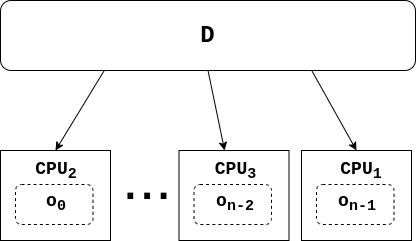
\includegraphics[width=0.65\linewidth]{figuras/procesamiento_paralelo_con_paralelizacion_func.png}
  \caption{Aplicación con paralelización de funciones}
  \label{fig:con_paralelizacion_funciones}
\end{figure}
